\chapter{Fundamentals} % Main chapter title
\label{chap:fund}

% Hier muss alles rein was benötigt wird um die Arbeit zu verstehen.
%   Man kann ja sicherlich grundlegendes Verständis von Recherstrukturen und Organisation vorraussetzten
%   Was also sollte definitiv nochmal erklärt werden?
%
%   - Virtual Memory -> Und vor allem die Kosten, das ist ja auch irgendwo der Aufhänger
%           Der Satz, "tlb is on the critical path of everything really" sollte irgendwann mal kommen
%   - Motivation für vm
%   - Organisationsstrukturen auch im vergleich -> Fazit: Page Tables sind überall und werden tiefer -> vor allem wegeb backwards compatiblity?
%   - Hardware Strukturen für VM - MMU, TLB
%   - Operating system and VM -> Implemented by OS but fixed structures given by MMU
%   -> Problem, fehlende flexibilität ->  A look at several ...
%   -> source: Architectural and operating system support for virtual memory
%   source: issues of implementation

\section{Virtual Memory}

% VM Properties and benefits: Was für Nutzen hat VM?
- idealized abstraction of storage resources available on a machine
- virtual to physical mapping
- flexibility to place actual data anywhere on the available disk
- emulate bigger memory than actually available
- foundation for isolation/security
- Implement flexible paging the swap pages between main memory and secondary storage
% Fazit: VM hat sehr nützliche Eigenschaften

% -----------------------------------------------------------------------

% Wie können wir VM realisieren? -> Verschiedene Implementationen, Aber hier nicht auf die HW eingehen
%   [ A look at several...]
%   [ Issues of implementation]
% \section{Implementation of Virtual Memory Systems}
% \subsection{ Overview of different implementations (Inverted/Hierarchical/Multi-Level)}
% \subsection{ Comparison of differnt implementations with regards to performance and features like page sharing}

% -> Most commonly used in todays hardware -> Multi level page tables
\begin{figure*}[t]
    \centering
    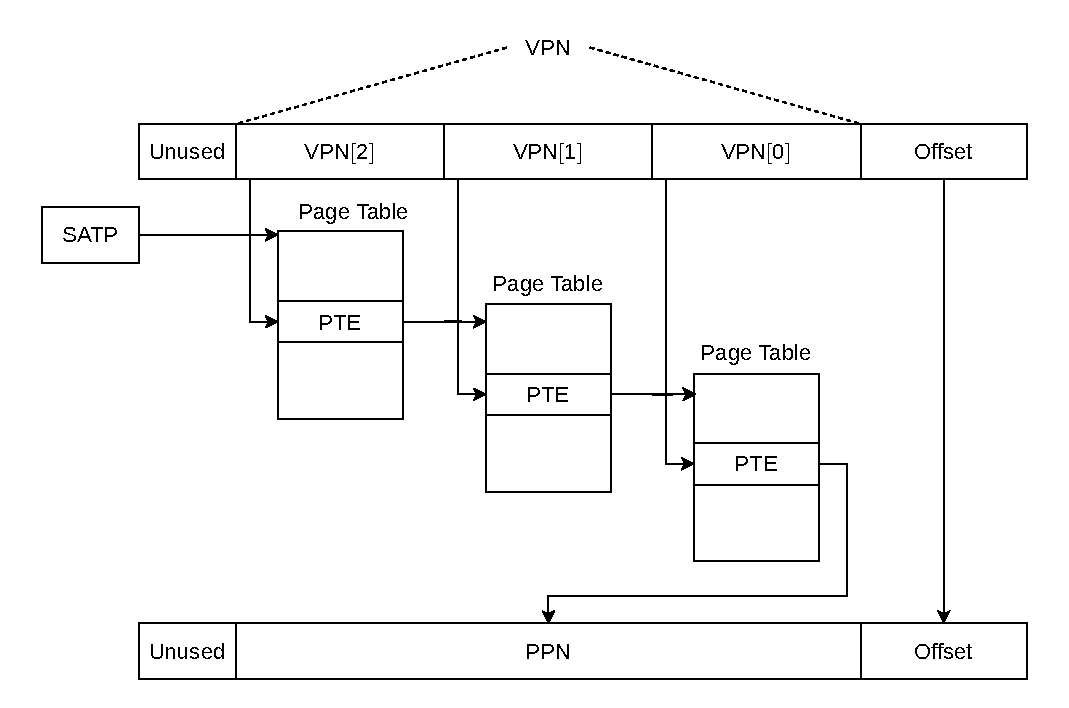
\includegraphics[scale=.8]{figures/VM-Tree.pdf}
    \caption[RISC-V Sv39 3-Level Page Tree]{RISC-V Sv39 3-Level Page Tree}
    \label{fig:fund:pagetree}
\end{figure*}

% Fazit -> Hauptproblem von VM sind teure Hauptspeicherzugriffe im kritischen Pfade von allen Memory Operations

% -----------------------------------------------------------------------

% Hardware Strukturen zur beschleunigung von VM
% \section{Hardware support}

\begin{figure*}[t]
    \centering
    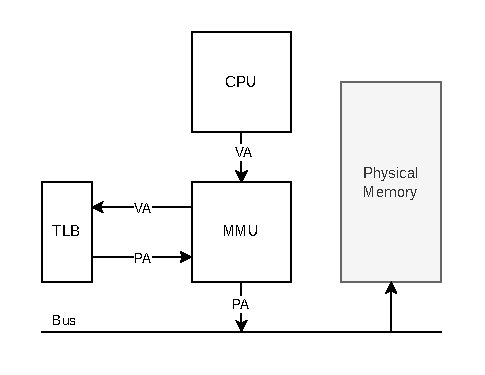
\includegraphics[]{figures/simple_mmu_arch.pdf}
    \caption[A simplified architecture of CPU, MMU and TLB]{A simplified architecture of CPU, MMU and TLB}
    \label{fig:fund:simplearch}
\end{figure*}

% \subsection{MMU & TLB}

% With only software ptw process would have to context switch to the kernel -> Very expensive
% With an MMU the processor essentially just freezes until the memory operation has completed
\cite{jacobVirtualMemoryContemporary1998}
% \subsection{HW-Dependent PTE Structure} -> inflexibility
% \subsection{A typical Page Table Walk}



% Fazit -> Es gibt hardware strukturen die VM beschleunigen können, die machen es auch schneller
%       ABER: Die machen die VM Software Systeme auch sehr viel rigider und unflexibler

% -----------------------------------------------------------------------

% VM in Software möglich mit ähnlicher Performance wie hw möglich -> Sollte ja mehr Flexibilität geben
%   [ A look at several...]
% \section{ Sofware VM Approaches}
% \section{ Liedtke GPTs}
% \subsection{More flexibilty}

% related work will then come in to discuss approaches close to my approach

